\section{Projekt systemu}
\begin{center}
	\label{img:system}
	\adjustbox{valign=t}{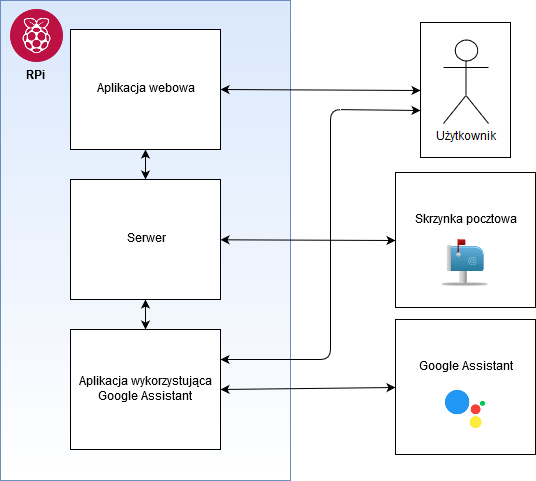
\includegraphics[width=12cm]{schemat.png}}
\end{center}
Rysunek \ref{img:system} przedstawia ogólny schemat opisywanego projektu.
Jego kolejne części są opisane w poniższych sekcjach:
\begin{itemize}
\item część RPI + Google Assistant w sekcji \textit{Raspberry Pi - Google Assistant}
\item część z ESP8266 w sekcji \textit{ESP8266}
\item serwer w sekcji \textit{Serwer}
\item aplikacja webowa w sekcji \textit{Aplikacja webowa}
\end{itemize}


\section{Raspberry Pi - Google Assistant}

Głównym elementem naszego projektu jest mikrokomputer Raspberry Pi 3 w wersji B. Zostanie na nim zainstalowany serwer aplikacji webowej (omówiony w rozdziale <tu wstaw rozdział> i Google Assistant. W niniejszej części dokumentu zostanie omówiony projekt bezpośredniego połączenia Raspberry Pi z urządzeniami zewnętrznymi (takimi jak głośnik, mikrofon) stanowiącymi razem pewną integralną całość, w założeniu mającą znaleźć się w jednej obudowie. Zdalny moduł wykorzystujący ESP8266 zostanie omówiony w innej części tego dokumentu.

\begin{center}
	\label{img:google}
	\adjustbox{valign=t}{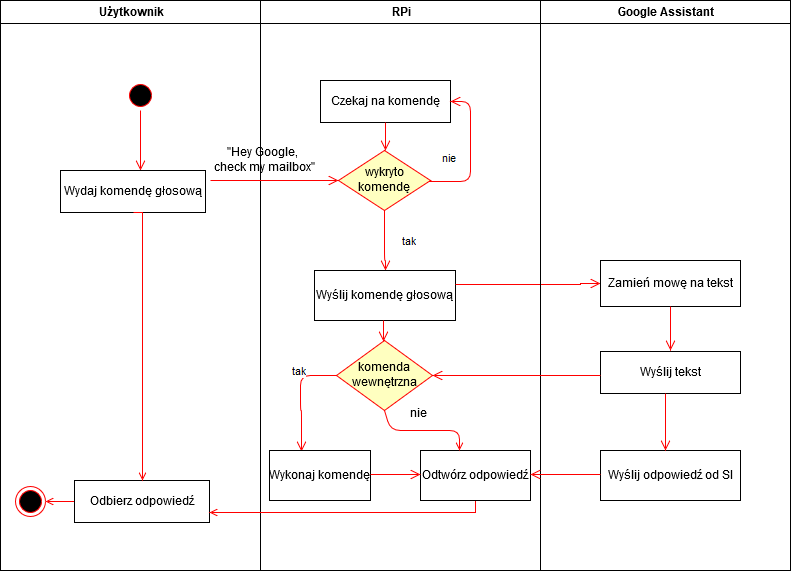
\includegraphics[width=14cm]{google.png}}
\end{center}
Rysunek \ref{img:google} przedstawia schemat części opartej o RPI i Google Assistanta.

\subsection{Spis urządzeń}

	\begin{figure}[H]
	\centering
	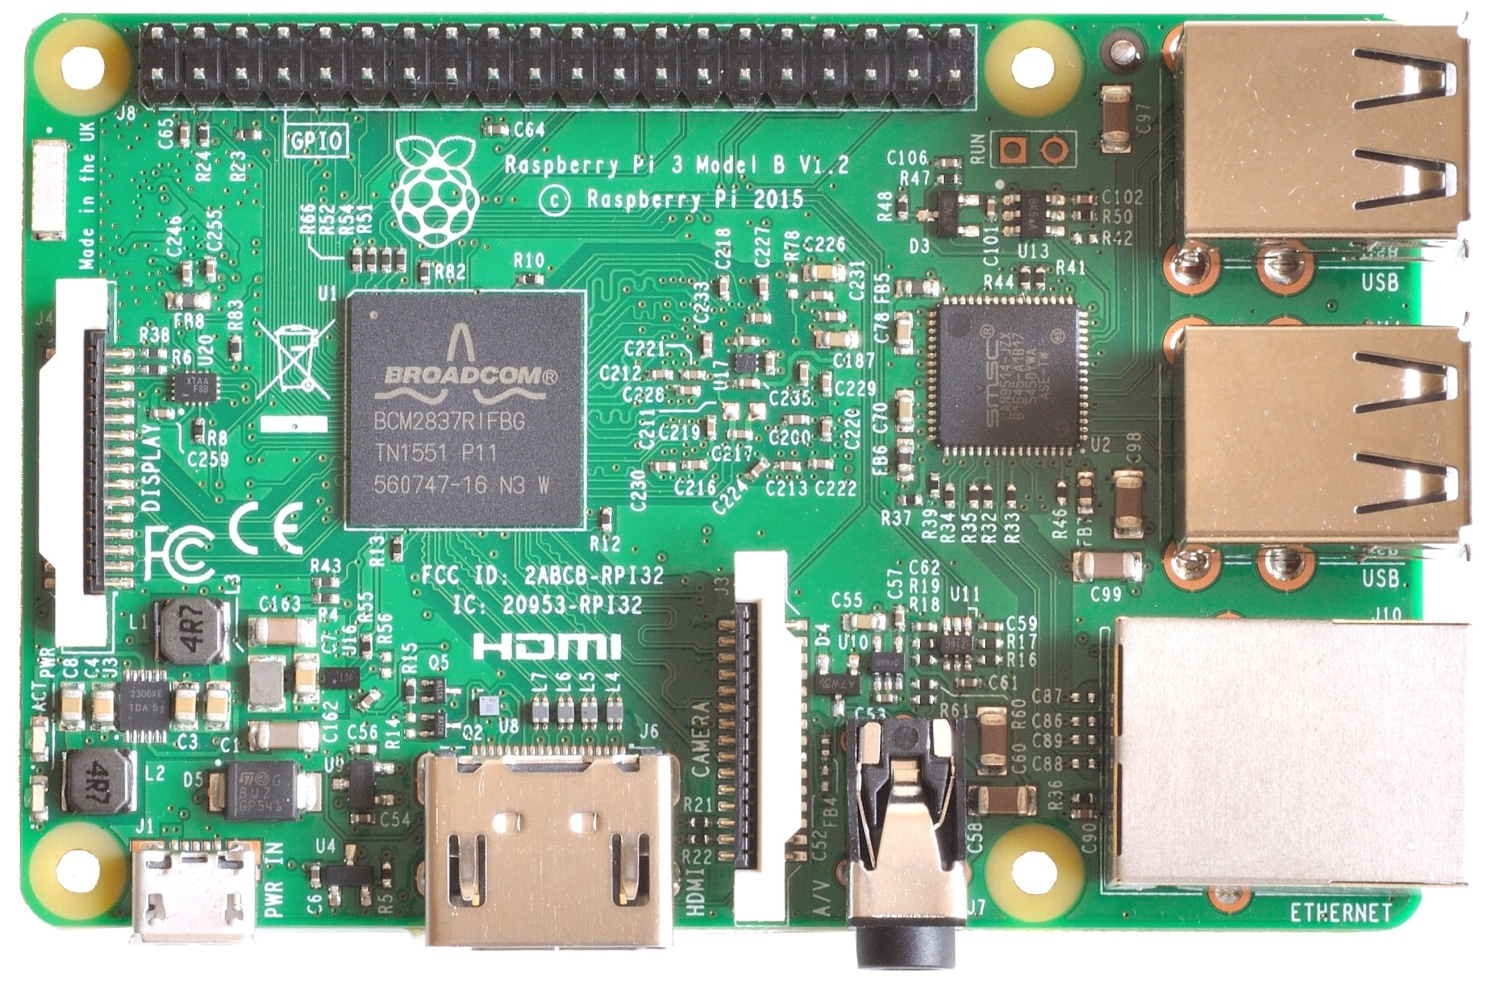
\includegraphics[width=8cm]{rpi.jpg}
	\caption{Raspberry Pi 3 w wersji B}
	\end{figure}
	
	\begin{figure}[H]
	\centering
	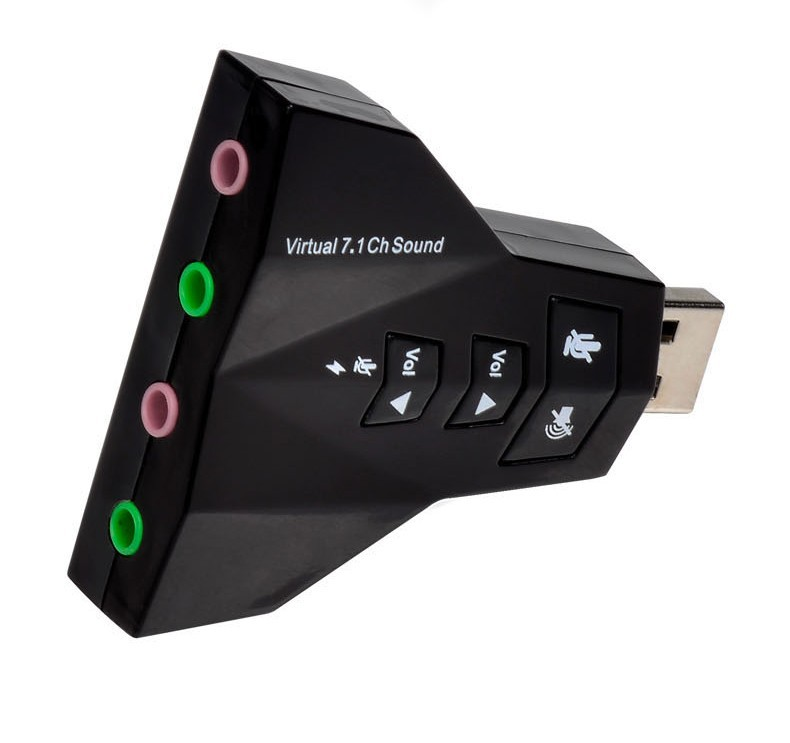
\includegraphics[width=8cm]{karta_muzyczna.jpg}
	\caption{Zewnętrzna karta dżwiękowa Virtual 7.1 Channel USB }
	\end{figure}
	
	\begin{figure}[H]
	\centering
	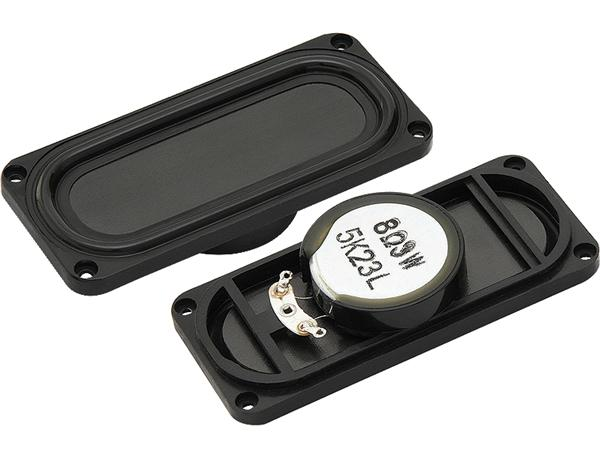
\includegraphics[width=8cm]{glosnik.jpg}
	\caption{Głośnik 3W 8Ohm 40x88mm}
	\end{figure}
	
	\begin{figure}[H]
	\centering
	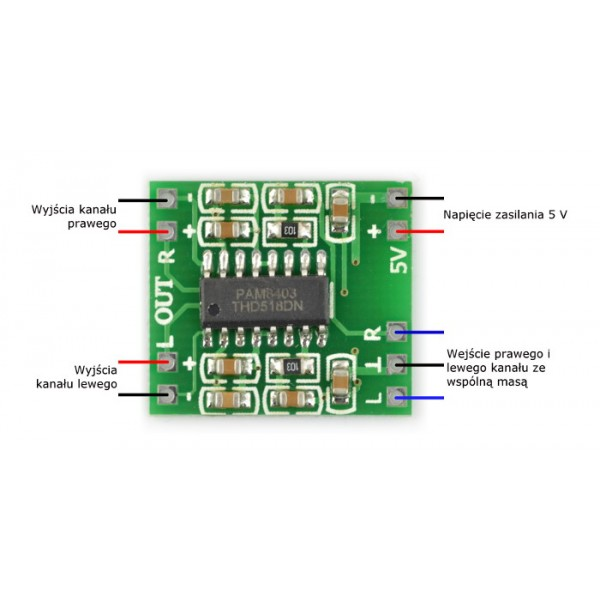
\includegraphics[width=8cm]{wzmacniacz.jpg}
	\caption{Wzmacniacz audio stereo PAM8403 5V 3W - dwukanałowy}
	\end{figure}
	
	\begin{figure}[H]
	\centering
	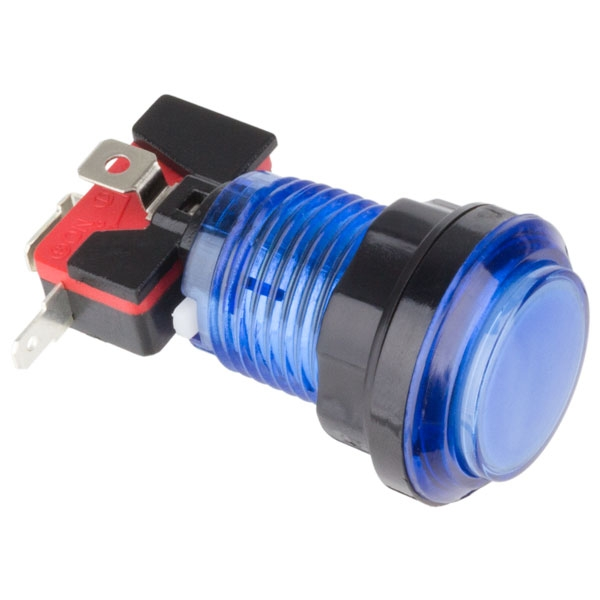
\includegraphics[width=8cm]{button.jpg}
	\caption{Rrzycisk Arcade Push Button niebieski z podświetleniem}
	\end{figure}

Dodatkowo zostanie wykorzystany mikrofon wykorzystujący złącze typu \emph{mini jack}.

\subsection{Schemat połączeń}

Na poniższym schemacie zaprezentowano układ połączeń wyżej wymienionych elementów. Rezystancje oporników mogą się różnić ze względu na wykorzystany tranzystor i rodzaj diody świecącej. W większości przypadków układ typu "klucz npn" nie będzie potrzebny, gdyż napięcie przewodzenia diody może okazać na tyle niskie, że będzie możliwe zasilenie jej z portu GPIO (niestety nie było tak w naszym przypadku).

\begin{center}
\adjustbox{valign=t}{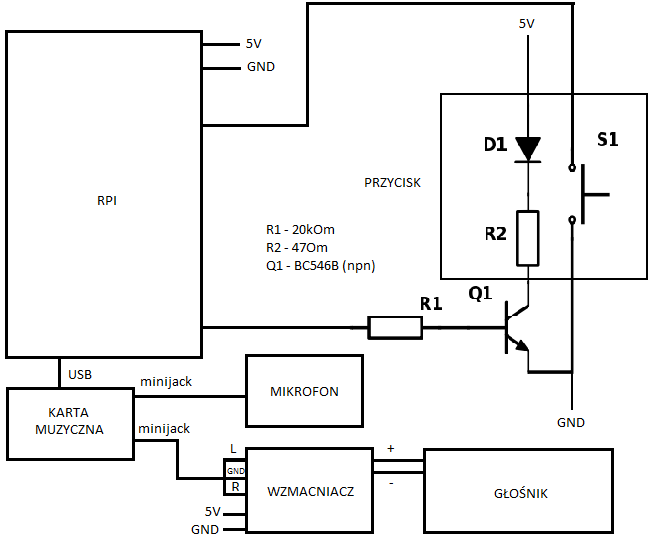
\includegraphics[width=8cm]{schematRPI.png}}
\end{center}


\section{ESP8266}

Drugim kluczowym elementem naszego projektu jest układ wykorzystujący moduł \emph{ESP8266}. Zostanie do niego podłączony nadajnik IR, odbiornik IR i bateria. Gdy odczyt sygnału, nadawanego przez pierwsze z urządzeń, nie będzie możliwy, znaczy to, że na drodze wiązki znajduje się jakaś przeszkoda - w założeniach ma to być list. Moduł zostanie oprogramowany tak aby, co jakiś ustalony czas, wysyłać do serwera informacje o odczycie. W finalnej wersji układ ma zostać zamontowany w skrzynce.
\subsection{Spis urządzeń}



	\begin{figure}[H]
	\centering
	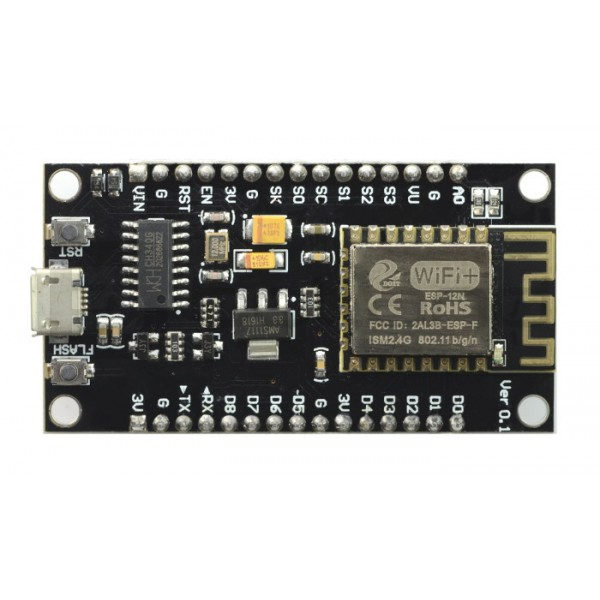
\includegraphics[width=7cm]{esp8266-nodemcu-v3.jpg}
	\caption{ESP8266 z ModeMCU v3}
	\end{figure}
	
	\begin{figure}[H]
	\centering
	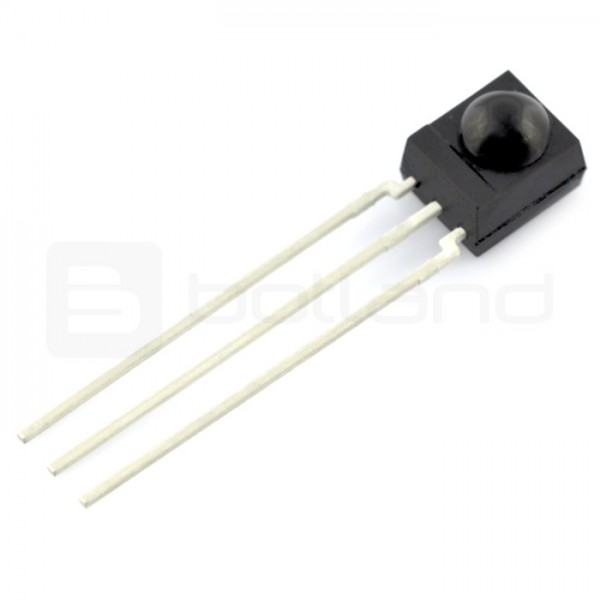
\includegraphics[width=7cm]{tsop4836.jpg}
	\caption{Odbiornik TSOP4836 }
	\end{figure}
	
	
	\begin{figure}[H]
	\centering
	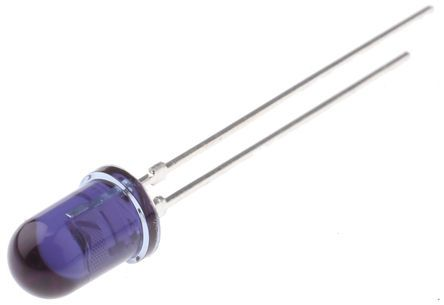
\includegraphics[width=7cm]{LIRED5C.jpg}
	\caption{Nadajnik IR LIRED5C}
	\end{figure}

\subsection{Schemat połączeń}

Poniższy schemat przedstawia układ połączeń wyżej wymienionych elementów. Warto zwrócić uwagę na połączenie pinu GPIO\_16 z pinem REST. Pozwoli to przełączać moduł ESP w tryb głębokiego snu - pozwoli to na oszczędzanie baterii.

\begin{center}
	\adjustbox{valign=t}{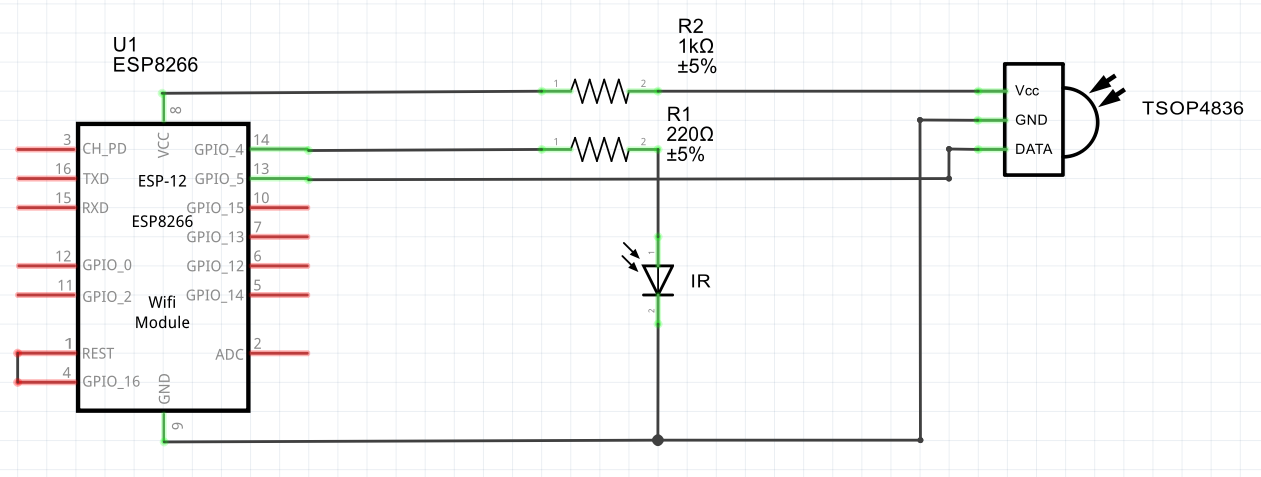
\includegraphics[width=8cm]{schematWiFI_IR.png}}
\end{center}

\section{Serwer}

Następną częścią projektu jest serwer oparty o technologię \textit{Flask}. Pozwala on na komunikację pomiędzy \textit{ESP8266}, \textit{Google Assistantem} oraz aplikacją webową.\\

Serwer jest uruchamiany na \textit{Raspberry PI}, na porcie 5000 i udostępnia klientom dwa \textit{endpointy}. Jeden z nich pozwala na pobranie aktualnego stanu skrzynki pocztowej, drugi - na jego zmianę. \\

REST API udostępniane przez serwer jest przedstawione w tabeli \ref{tab:api}.

\begin{longtable}{|c|c|c|p{4cm}|}
\caption{Serwer REST API} \label{tab:api} \\ \hline
\multicolumn{4}{ |c| }{ Skrzynka pocztowa } \\ \hline
\multicolumn{4}{ |c| }{ /state } \\ \hline
Endpoint & Request & Opis & Dodatkowo \\ \hline
/state & GET & Pobranie informacji o stanie skrzynki & Rezultat: 0 - pusta skrzynka, 1 - pełna \\ \hline
/state/[state] & POST & Zmiana stanu na [state] & state może przyjąć wartości: 0 lub 1 \\ \hline
\end{longtable} 

\begin{center}
	\label{img:serwer_class}
	\adjustbox{valign=t}{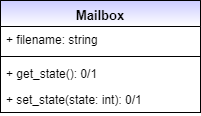
\includegraphics[width=6cm]{serwer_class.png}}
\end{center}

Serwer korzysta z klasy Mailbox, która udostępnia dwie metody: do pobrania stanu skrzynki i do ustawienia stanu skrzynki. Więc o obu metodach można znaleźć w rozdziale 5 \textit{Realizacja}. Diagram klasy jest widoczny na rysunku \ref{img:serwer_class}

Stan skrzynki jest zapisywany w pliku, w postaci:
\begin{itemize}
\item 0 - gdy skrzynka jest pusta
\item 1 - gdy w skrzynce mamy jakieś wiadomości
\end{itemize}

W przypadku, jeśli na \textit{Raspberry PI} nie ma wymaganych przez serwer zależności (Flask w wersji 0.10.1) należy wywołać:
\begin{lstlisting}
pip install -r requirements.txt
\end{lstlisting}

Uruchamianie serwera następuje przez wywołanie:
\begin{lstlisting}
python run.py
\end{lstlisting}


\section{Aplikacja webowa}

\begin{center}
	\label{img:skrzynka}
	\adjustbox{valign=t}{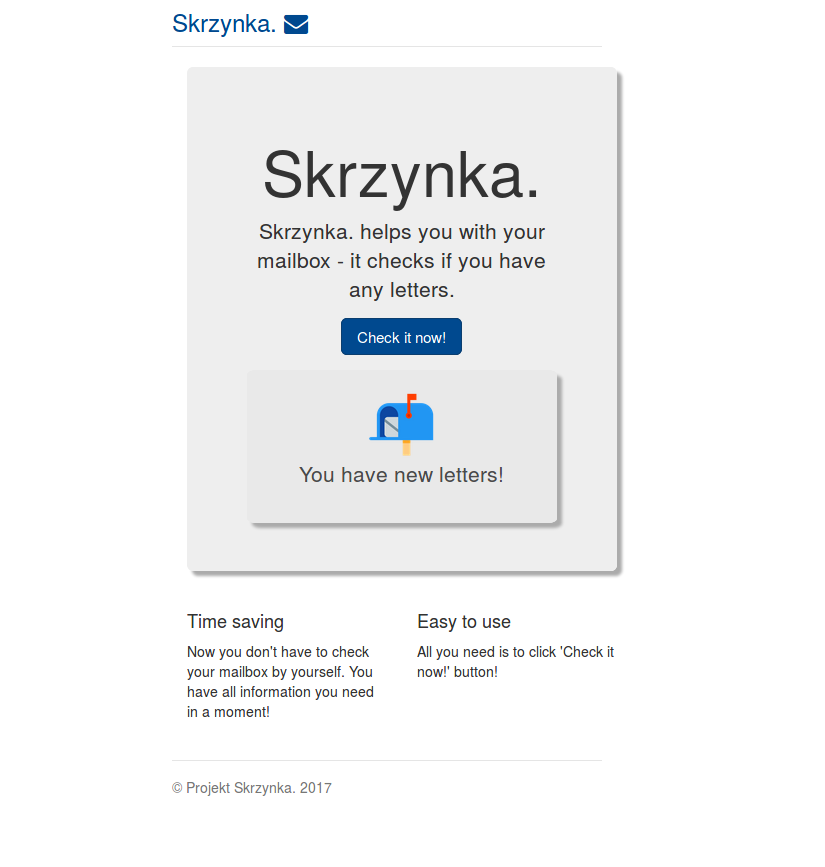
\includegraphics[width=10cm]{skrzynka2.png}}
\end{center}

Aplikacja webowa pozwala na sprawdzenie aktualnego stanu skrzynki pocztowej. Jest widoczna na rysunkach \ref{img:skrzynka}.
Logika aplikacji została stworzona w języku \textit{Java Script} wraz z \textit{AngularJS}, natomiast widok to \textit{HTML5} wraz z arkuszami stylów (\textit{CSS}).\\

Składa się z trzech głównych części:
\begin{itemize}
\item widoku - który określa elementy, jakie są obecne na stronie
\item kontrolera - który odpowiada za logikę w aplikacji (wykorzystuje serwis do wysyłania zapytań do serwera)
\item serwisu - który wysyła zapytanie \textbf{GET /state} na adres serwera
\end{itemize}

Na stronie dostępny jest przycisk \textbf{Check it now!} (ang. \textit{Wypróbuj już teraz!}), który wywołuje metodę kontrolera odpowiedzialną za wykonanie zapytania do serwera przez serwis.

\begin{center}
	\label{img:web_diagram}
	\adjustbox{valign=t}{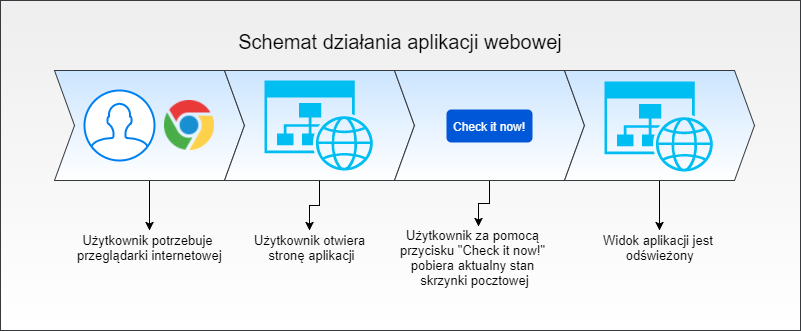
\includegraphics[width=14cm]{web_diagram.png}}
\end{center}

Rysunek przedstawiony wyżej (\textit{Schemat działania aplikacji webowej}) przedstawia schemat działania aplikacji webowej.

Uruchomienie serwera \textit{node.js} z parametrem wskazującym na ścieżkę do pliku \textbf{server.js}:
\begin{lstlisting}
node server.js
\end{lstlisting}

W przypadku, jeśli na \textit{Raspberry PI} nie ma wymaganych przez aplikację zależności należy wywołać:
\begin{lstlisting}
bower install
npm install connect
npm install serve-static
\end{lstlisting}
i później uruchomić serwer \textit{node.js}.
%
%	\begin{figure}
%	\centering
%	\label{img:skrzynka2}
%	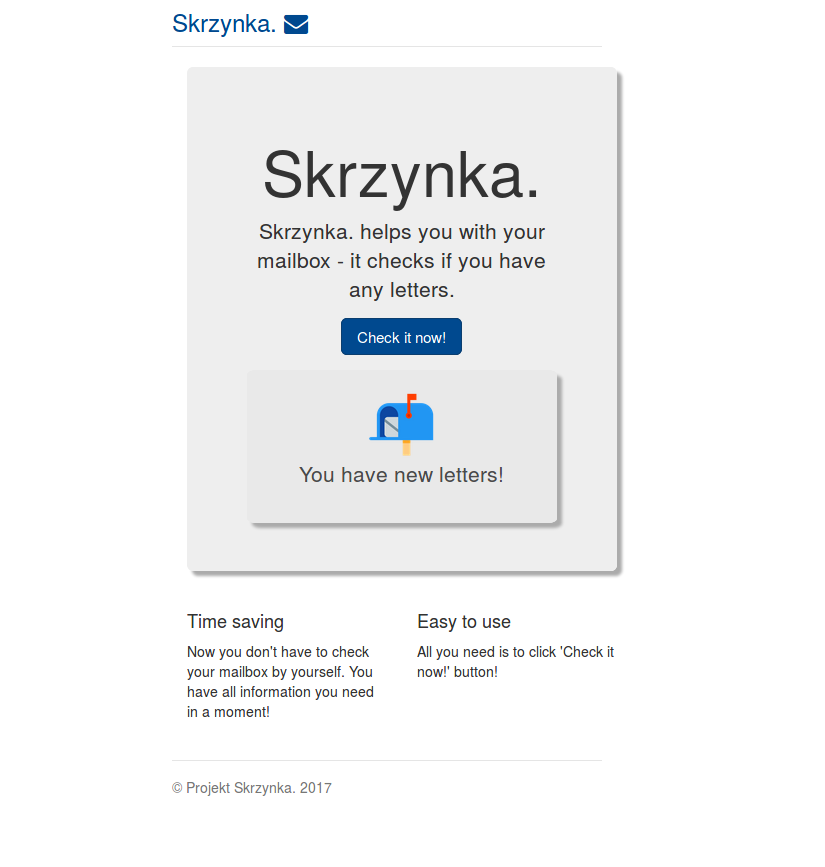
\includegraphics[width=10cm]{skrzynka2.png}
%	\caption{skrzynka2}
%	\end{figure}

